\section{Experimental Evaluation}\label{sec:eval}

\begin{figure}[t]
  \begin{adjustwidth}{-0.13\textwidth}{-0.13\textwidth}
  	\centering
    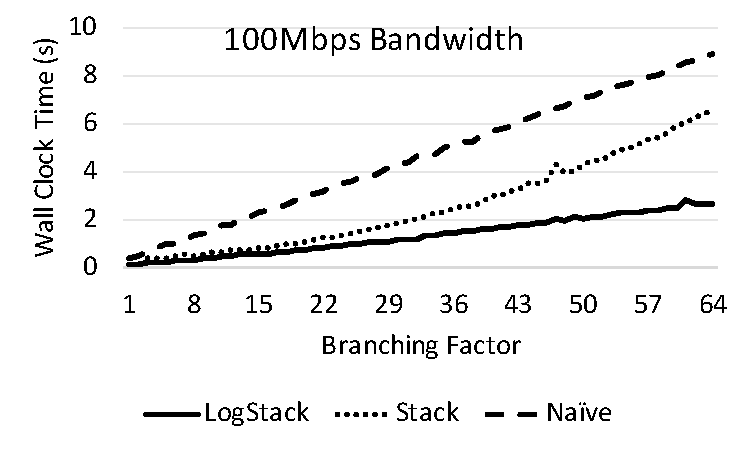
\includegraphics[width=0.4\textwidth]{fig/100mbps}
    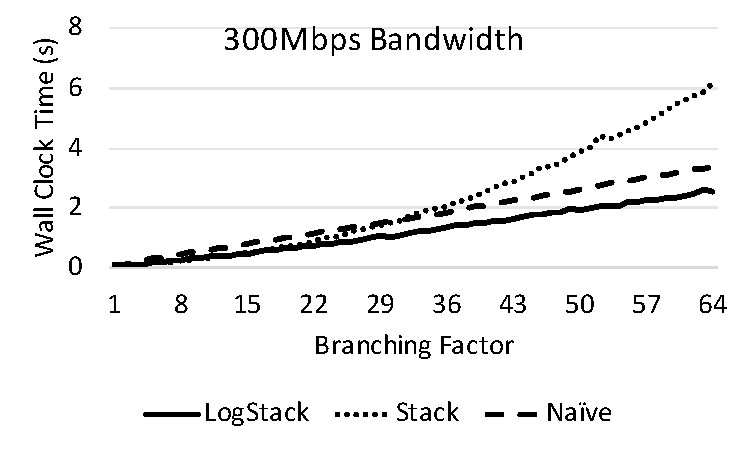
\includegraphics[width=0.4\textwidth]{fig/300mbps}
    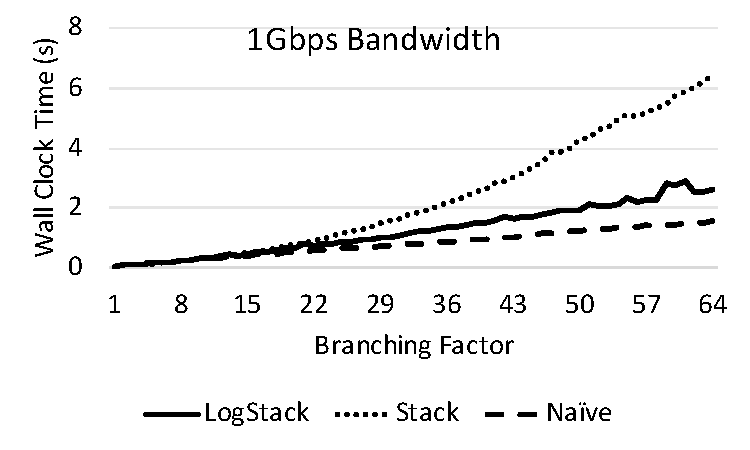
\includegraphics[width=0.4\textwidth]{fig/1gbps}
  	\\
    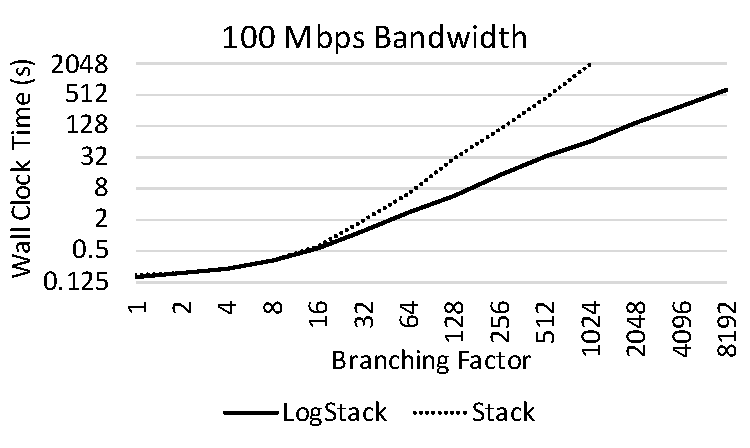
\includegraphics[width=0.4\textwidth]{fig/highbranching}
    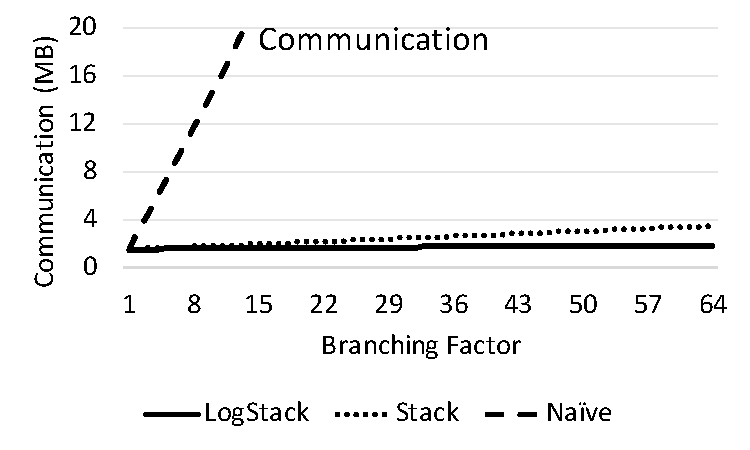
\includegraphics[width=0.4\textwidth]{fig/comm}
    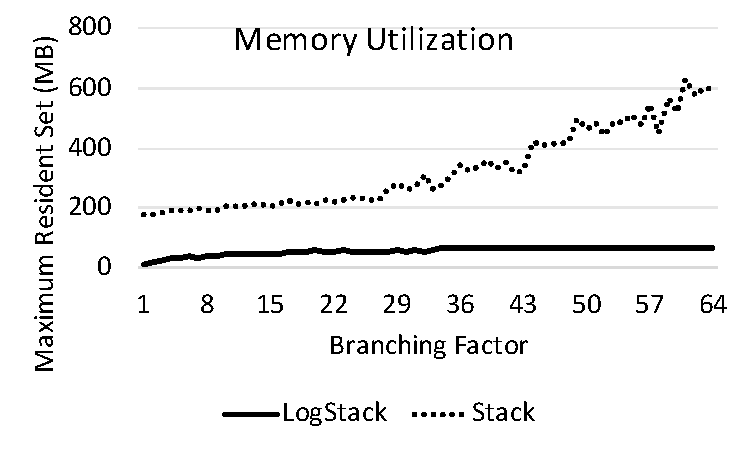
\includegraphics[width=0.4\textwidth]{fig/memutil}
  \end{adjustwidth}
  \caption{%
  }\label{fig:plots}
\end{figure}

We implemented \ourschemelong and extensively experimented with it and with implementations of basic half-gates~\cite{EC:ZahRosEva15} and the \stack SGC of~\HK.
We report on our experimental evaluation, and compare in detail to  basic half-gates~\cite{EC:ZahRosEva15} and to~\HK.

We address the following metrics: end-to-end wall-clock time performance of the 2PC implemented with each of the three schemes.